\tikzset{every picture/.style={line width=0.75pt}} %set default line width to 0.75pt        

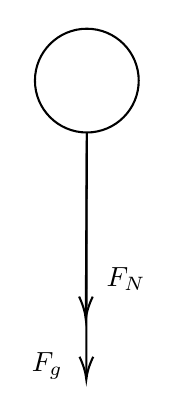
\begin{tikzpicture}[x=0.75pt,y=0.75pt,yscale=-1,xscale=1]
%uncomment if require: \path (0,300); %set diagram left start at 0, and has height of 300

%Shape: Circle [id:dp5520731613008669] 
\draw   (171,145) .. controls (171,131.19) and (182.19,120) .. (196,120) .. controls (209.81,120) and (221,131.19) .. (221,145) .. controls (221,158.81) and (209.81,170) .. (196,170) .. controls (182.19,170) and (171,158.81) .. (171,145) -- cycle ;
%Straight Lines [id:da12065599323998066] 
\draw    (196,170) -- (195.51,258) ;
\draw [shift={(195.5,260)}, rotate = 270.32] [color={rgb, 255:red, 0; green, 0; blue, 0 }  ][line width=0.75]    (10.93,-3.29) .. controls (6.95,-1.4) and (3.31,-0.3) .. (0,0) .. controls (3.31,0.3) and (6.95,1.4) .. (10.93,3.29)   ;
%Shape: Boxed Line [id:dp90095876721953] 
\draw    (196,170) -- (195.75,287) ;
\draw [shift={(195.75,289)}, rotate = 270.12] [color={rgb, 255:red, 0; green, 0; blue, 0 }  ][line width=0.75]    (10.93,-3.29) .. controls (6.95,-1.4) and (3.31,-0.3) .. (0,0) .. controls (3.31,0.3) and (6.95,1.4) .. (10.93,3.29)   ;

% Text Node
\draw (204,233.4) node [anchor=north west][inner sep=0.75pt]    {$F_{N}$};
% Text Node
\draw (168,274.4) node [anchor=north west][inner sep=0.75pt]    {$F_{g}$};


\end{tikzpicture}
